\documentclass[t]{beamer}
%\usepackage{multimedia}		% for movies, sounds, animations...
\usepackage[ngerman,german,english]{babel}		% new german
\usepackage[utf8]{inputenc}		% input...

\usepackage{tabularx}			% local, only for this doc.
\usepackage{hyperref}
\usepackage[tamsWZ, blockBG, tams,engl]{tamsBeamer}

\usepackage{listings}
  % Listingsformatierung (Quelltexte)
\definecolor{lightgrey}{rgb}{0.90,0.90,0.90}

\lstset{
	tabsize=2,
	escapeinside={(*@}{@*)},
	captionpos=t,
	framerule=0pt,
	backgroundcolor=\color{lightgrey},
	basicstyle=\footnotesize\ttfamily,
	keywordstyle=\footnotesize\bfseries,
	numbers=left,
	fontadjust,
	breaklines=true,
	postbreak=\mbox{\textcolor{black}{$\hookrightarrow$}\space}
}

\newcommand{\vectwo}[2]{
	\left(
	\begin{matrix}
		#1 \\
		#2 
	\end{matrix}
	\right)
}

\newcommand{\vecthr}[3]{
	\left(
	\begin{matrix}
		#1 \\
		#2 \\
		#3
	\end{matrix}
	\right)
}
%-----------------------------------------------------------------------------
%-- options		------------------------------------------------------
%			tams	|	- TAMS		publication
%			cinacs		- CINACS	publication
%			engl		- english strings	[german]
%			uniWZ	|	- uni		watermark
%			tamsWZ	|	- tams+uni	watermark
%			cinacsWZ	- cinacs+uni	watermark
%			secToc	|	- toc repetition at each section
%			secTocA		- -"-, all sections: show
%					  replacement for toc in short docs
%			subsecToc	- toc repetition at each subsection
%			secNum  	- (sub)-section numbering
%			fullstep	- always step through items
%			noFoot		- footline	off
%			noPage		- page numbers	off
%			noAuth		- author	off
%			conference	- footline with \foottitle{...}
%			blockBG	|	- block, example etc. background
%			blockRound	- -"-, rounded+shadow


% fonts definitions			--------------------------------------
% ----------------------------------------------------------------------------
% default: cmss, OT1 fontenc		good with UniHH font "The Sans"
%					-> don't change fonts!
%\usepackage{times}			% other fonts
%\usepackage[T1]{fontenc}		%

% document definitions			--------------------------------------
% ----------------------------------------------------------------------------
\title		% title		-- option: short
  {Multitouch Robot Control}
\subtitle[B.Sc. Thesis]			% subtitle	-- option: short
  {Bachelor Thesis}

\author[M.~Steuer]{Merlin Steuer}

%\author[AutorA, AutorB]		% author	-- option: short
% {A.~Autor\inst{1} \and B.~Autor\inst{2}}%		-- option: \inst{...}
% style option: [tams] predefines institute...
% or define \institute{...}
%					% \inst{...} for different institutions
%\institute[Universities A and B]	% institution	-- option: short
%{ \inst{1}%
%  University of A\\
%  Department of A
%  \and
%  \inst{2}%
%  University of B\\
%  Department of B}

\date[24-apr-2018]			% event/date	-- option: short
  {24.~April 2018}

%\subject{TAMS, LaTeX, Folien}		% subject	-- option for pdf

% detailed information to be embedded in PDF		------------------- --
%\hypersetup{%
%  pdftitle={TAMS-Folien mit 'beamer'},
%  pdfauthor={Andreas Mäder, Universität Hamburg,
%        MIN-Fakultät, Fachbereich Informatik, TAMS},
%  pdfsubject={Präsentationen mit pdflatex erstellen},
%  pdfkeywords={TAMS, LaTeX, Folien}}


\usepackage[backend=bibtex8,
style=numeric,
citestyle=numeric,
alldates=edtf,
maxbibnames=99]{biblatex}

\addbibresource{Bachelorarbeit.bib}  
\renewcommand*{\bibfont}{\footnotesize}

% document starts here			--------------------------------------
% ----------------------------------------------------------------------------
\begin{document}

% titlepage				--------------------------------------
%\frame[plain]{\titlepage}		% suppress head- and footlines
\frame{\titlepage}

% toc					--------------------------------------
\begin{frame}[allowframebreaks]
  \frametitle{\tocName}
  \tableofcontents
  %\tableofcontents[pausesections]	% step through sections
\end{frame}

\section{Introduction}

\begin{frame}{Merlin Steuer}
\begin{itemize}
	\item Part-time student
	\item B.Sc. Informatik since WiSe13
	\item 2steuer@informatik.uni-hamburg.de
	\item Questions? Make some noise!
\end{itemize}
\end{frame}

\subsection{Motivation \& Objective}

\begin{frame}{Motivation \& Objective}
\begin{itemize}
	\item Robots get more and more ubiquitous
	\item Robots enter domestic space\cite{Forlizzi2006}
	\item Interfaces have to be easy and intuitive
\end{itemize}

$\Rightarrow$ A simple, intuitive remote control interface to complex robots shall be developed.

\begin{itemize}
	\item Multitouch gestures well known
	\item Android tablet computer
\end{itemize}
\end{frame}

\begin{frame}{Grasp Synergies}
\begin{itemize}
	\item Research at the TAMS group \cite{Bernardino2013}
	\item PCA on human grasp postures
	\item Eigenvectors in matrix $S$ (called \textit{Synergy} here)
	\item Offset $s_0$~$=$~mean joint values 
\end{itemize}

\begin{equation}
\theta = s_0 + S\alpha
\end{equation}

\begin{itemize}
	\item $\alpha \in \mathbb{R}^{21}$\quad input amplitudes
	\item $\theta \in \mathbb{R}^{21}$\quad joint angles of the hand
\end{itemize}

$\Rightarrow$ Map properties of gestures to $\alpha$ (Absolute and relative)

\end{frame}

\begin{frame}{Grasp Synergies}
\begin{figure}
	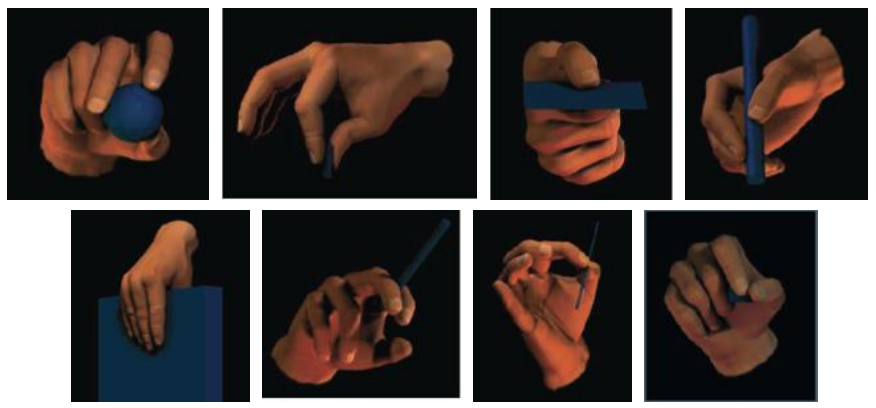
\includegraphics[height=0.6\textheight]{assets/pres/grasps.PNG}
	\caption{Grasp synergies recorded by \citeauthor{Bernardino2013}\cite{Bernardino2013}}
\end{figure}
\end{frame}

\begin{frame}{Direct Fingertip Mapping}
\begin{itemize}
	\item Research done by \citeauthor{conf:humanoids:TohHLBZP12} \cite{conf:humanoids:TohHLBZP12}
	\item Grasp actions $\rightarrow$ fingertip movements in a plane
\end{itemize}

$\Rightarrow$ Map fingertips on touch screen to a plane in $3D$ space
\end{frame}

\begin{frame}{Direct Fingertip Mapping}
\begin{figure}
	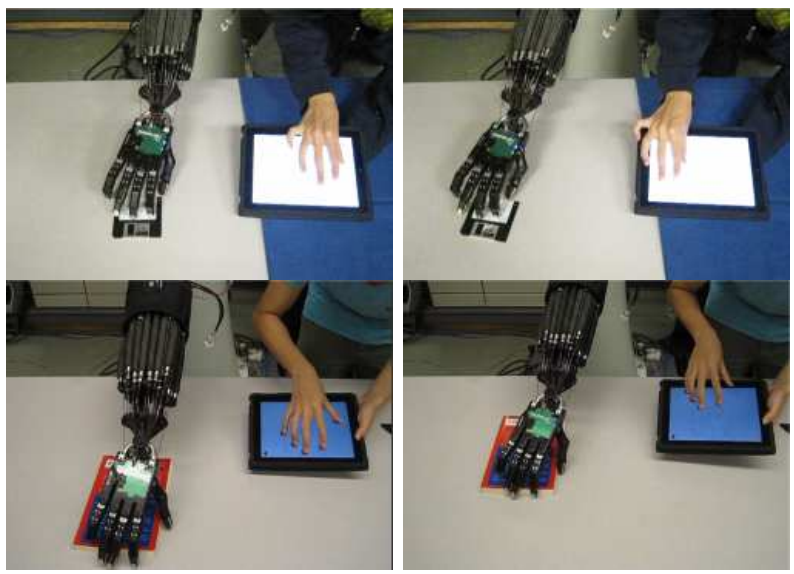
\includegraphics[height=0.6\textheight]{assets/pres/dftm_toh.PNG}
	\caption{Examples from \citeauthor{conf:humanoids:TohHLBZP12}\cite{conf:humanoids:TohHLBZP12}}
\end{figure}
\end{frame}

\subsection{Related Work}

\begin{frame}{Other Approaches}

\begin{minipage}{0.49\linewidth}
\begin{figure}
	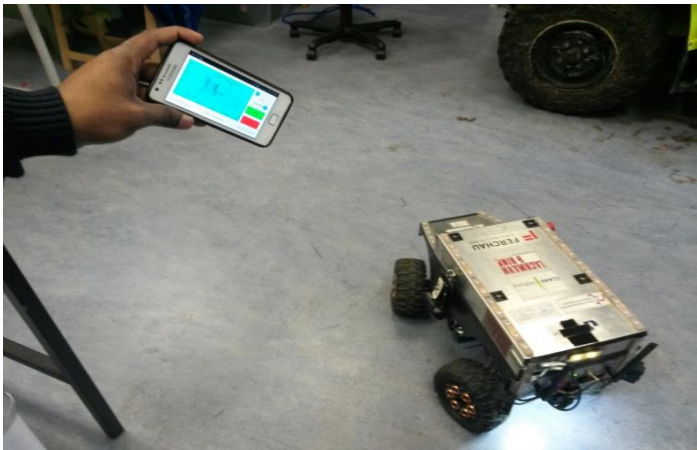
\includegraphics[width=\linewidth]{assets/pres/akupati.png}
	\caption{Controlling a robotic car with an Android phone, research by \citeauthor{Akupati2017}\cite{Akupati2017}}
\end{figure}
\end{minipage}
\begin{minipage}{0.49\linewidth}
\begin{figure}
	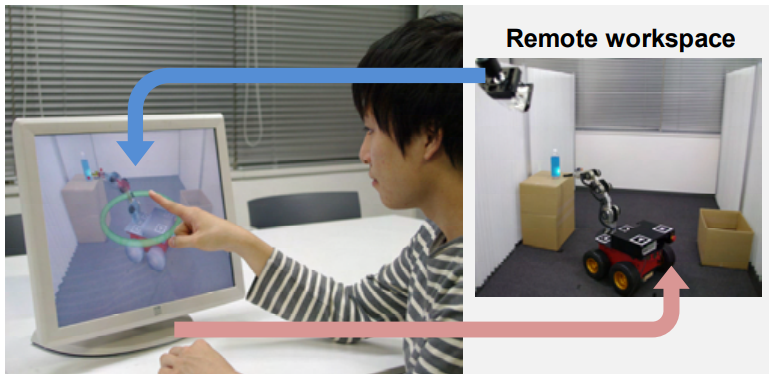
\includegraphics[width=\linewidth]{assets/pres/touchme.png}
	\caption{TouchMe! Controlling a robot with touch actions on an AR display. Research by \citeauthor{Hashimoto2013}\cite{Hashimoto2013}}
\end{figure}
\end{minipage}

\end{frame}

\subsection{Basics}

\begin{frame}{ROS}
\begin{itemize}
	\item Robot Operating System
	\item Software Framework to develop robots
	\item Communication Framework
	\item Publisher/Subscriber Pattern
	\item Services
\end{itemize}

\end{frame}

\begin{frame}{Inverse Kinematics}
\begin{itemize}
	\item Joint Space $\theta$
	\item Cartesian Space $x$
	\item Forward Kinematics: $x = f(\theta)$
	\item Inverse Kinematics: $\theta = f^{-1}(x)$
\end{itemize}

\begin{figure}
	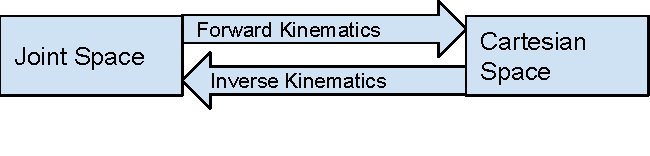
\includegraphics[scale=0.6]{assets/chpt_basics/Kinematics}
\end{figure}
\end{frame}

\subsection{Hardware}

\begin{frame}{Shadow C5 Hand}
\begin{minipage}{0.3\linewidth}
\begin{figure}
	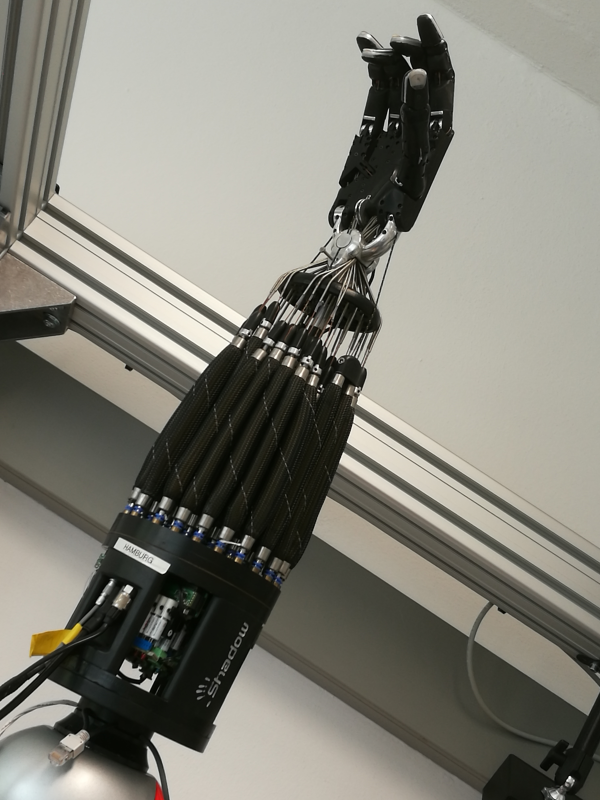
\includegraphics[width=\linewidth]{assets/chpt_basics/hand.png}
	\caption{The Shadow C5 Robotic Hand}
\end{figure}
\end{minipage}
\begin{minipage}{0.68\linewidth}
	\begin{itemize}
		\item by \textit{The Shadow Robot Company} \cite{web:robothand:spec}
		\item 24 DOF
		\item Pneumatic muscles
		\item Designed after human forearm
	\end{itemize}
\end{minipage}
\end{frame}

\begin{frame}{Kuka LWR 4+}
\begin{minipage}{0.45\linewidth}
	\begin{figure}
		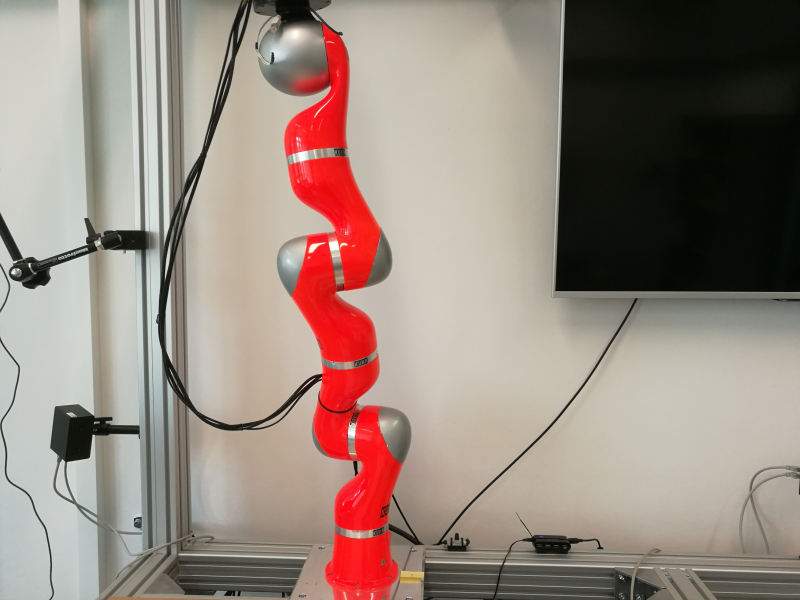
\includegraphics[width=\linewidth]{assets/chpt_basics/arm.png}
		\caption{The Kuka LWR robotic arm}
	\end{figure}
\end{minipage}
\begin{minipage}{0.5\linewidth}
	\begin{itemize}
		\item by \textit{KUKA Roboter GmbH} \cite{Lwr2010}
		\item 7 DOF
		\item Integration into ROS over FRI (\textit{Fast Research Interface})\cite{Fri2010}
	\end{itemize}
\end{minipage}
\end{frame}

\begin{frame}{Samsung Galaxy Tab S3}
\begin{minipage}{0.45\linewidth}
	\begin{figure}
		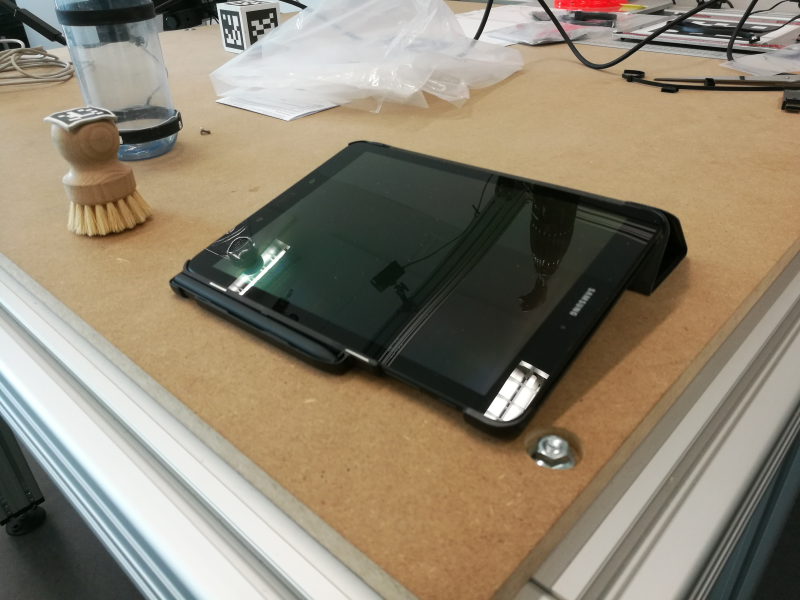
\includegraphics[width=\linewidth]{assets/chpt_concepts/tablet.png}
		\caption{The used Android tablet}
	\end{figure}
\end{minipage}
\begin{minipage}{0.5\linewidth}
	\begin{itemize}
		\item by \textit{Samsung} \cite{samsung:galaxytabs3}
		\item 10 inch screen
		\item 2048x1536 px
		\item 2.15GHz Quad-Core CPU
		\item \textit{rosjava} / \textit{rosandroid}
	\end{itemize}
\end{minipage}
\end{frame}

\subsection{BioIK}

\begin{frame}{BioIK}
\begin{itemize}
	\item Evolutionary, multi-goal algorithm for inverse kinematics
	\item Developed at the TAMS group \cite{Starke2017,Starkea2017}
	\item Integrated into ROS by Philipp Ruppel \cite{Ruppel17}
	\item Philipp also provided the BioIK ROS service\footnote{Found at \href{https://gogs.crossmodal-learning.org/philipp.ruppel/bio_ik_service}{Philipp's GOGS}}
\end{itemize}
\end{frame}

\section{User Interface}

\begin{frame}{User Interface}
\begin{itemize}
	\item Most area reserved for touch interaction
	\item Functionality interchangeable by tab pages
	\item Safety interlock button
	\item \textbf{Interlock button does not replace hardware safety measures!}
\end{itemize}
\end{frame}

\begin{frame}{User Interface}
\begin{figure}
	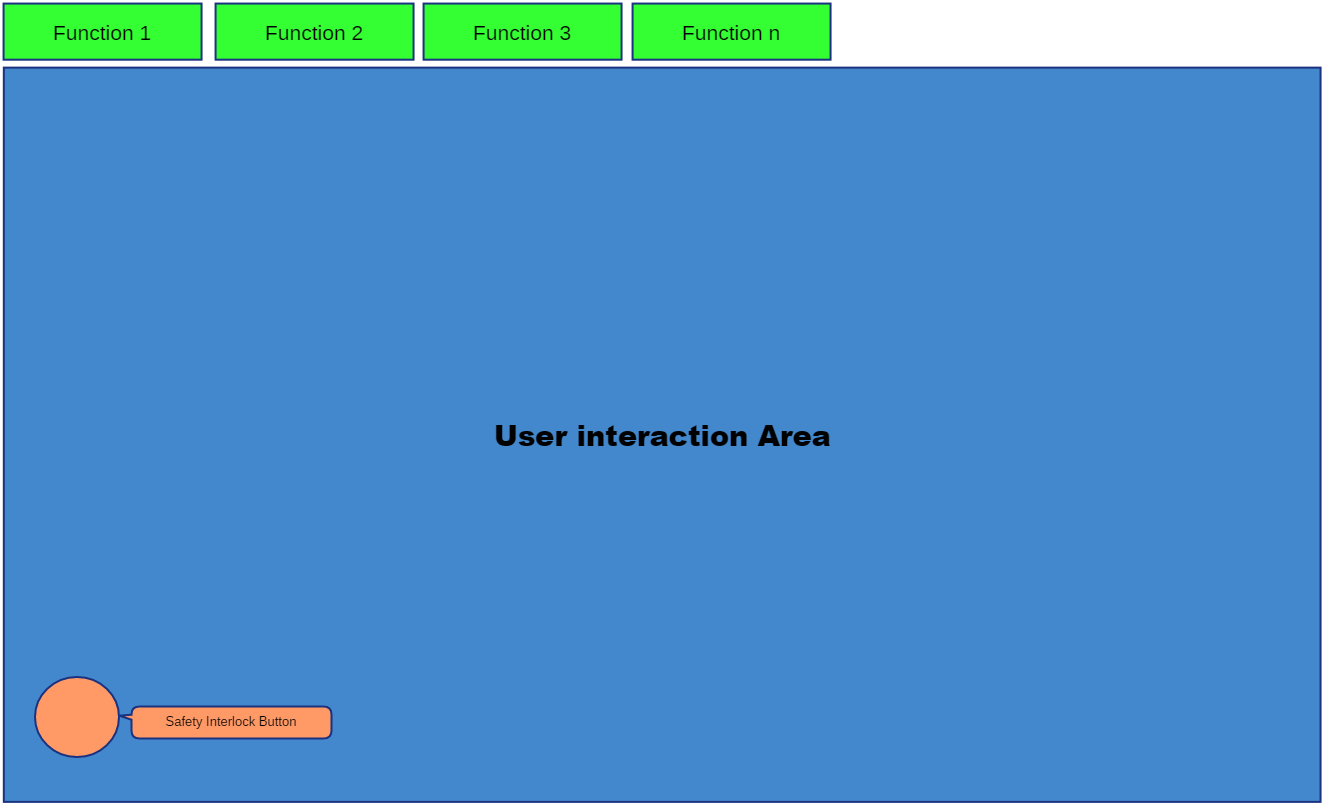
\includegraphics[width=0.8\linewidth]{assets/chpt_concepts/main_touch_interface.png}
	\caption{General screen layout}
\end{figure}
\end{frame}

\begin{frame}{Axis Control Page}
\begin{minipage}{0.55\linewidth}
\begin{itemize}
	\item One control for every joint
	\item +/- buttons to set joint angle
	\item Display of target value and current value
	\item Coloured indication of angle error
\end{itemize}
\end{minipage}
\begin{minipage}{0.4\linewidth}
	\begin{figure}
		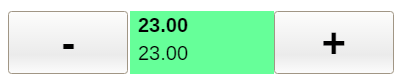
\includegraphics[width=\linewidth]{assets/chpt_concepts/AxisControlGreen.png}
		
		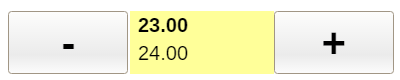
\includegraphics[width=\linewidth]{assets/chpt_concepts/AxisControlYellow.png}
		
		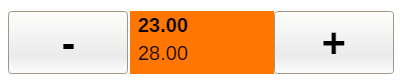
\includegraphics[width=\linewidth]{assets/chpt_concepts/AxisControlRed.png}
	\end{figure}
\end{minipage}
\end{frame}

\begin{frame}{Axis Control Page}
\begin{figure}
	\boxed{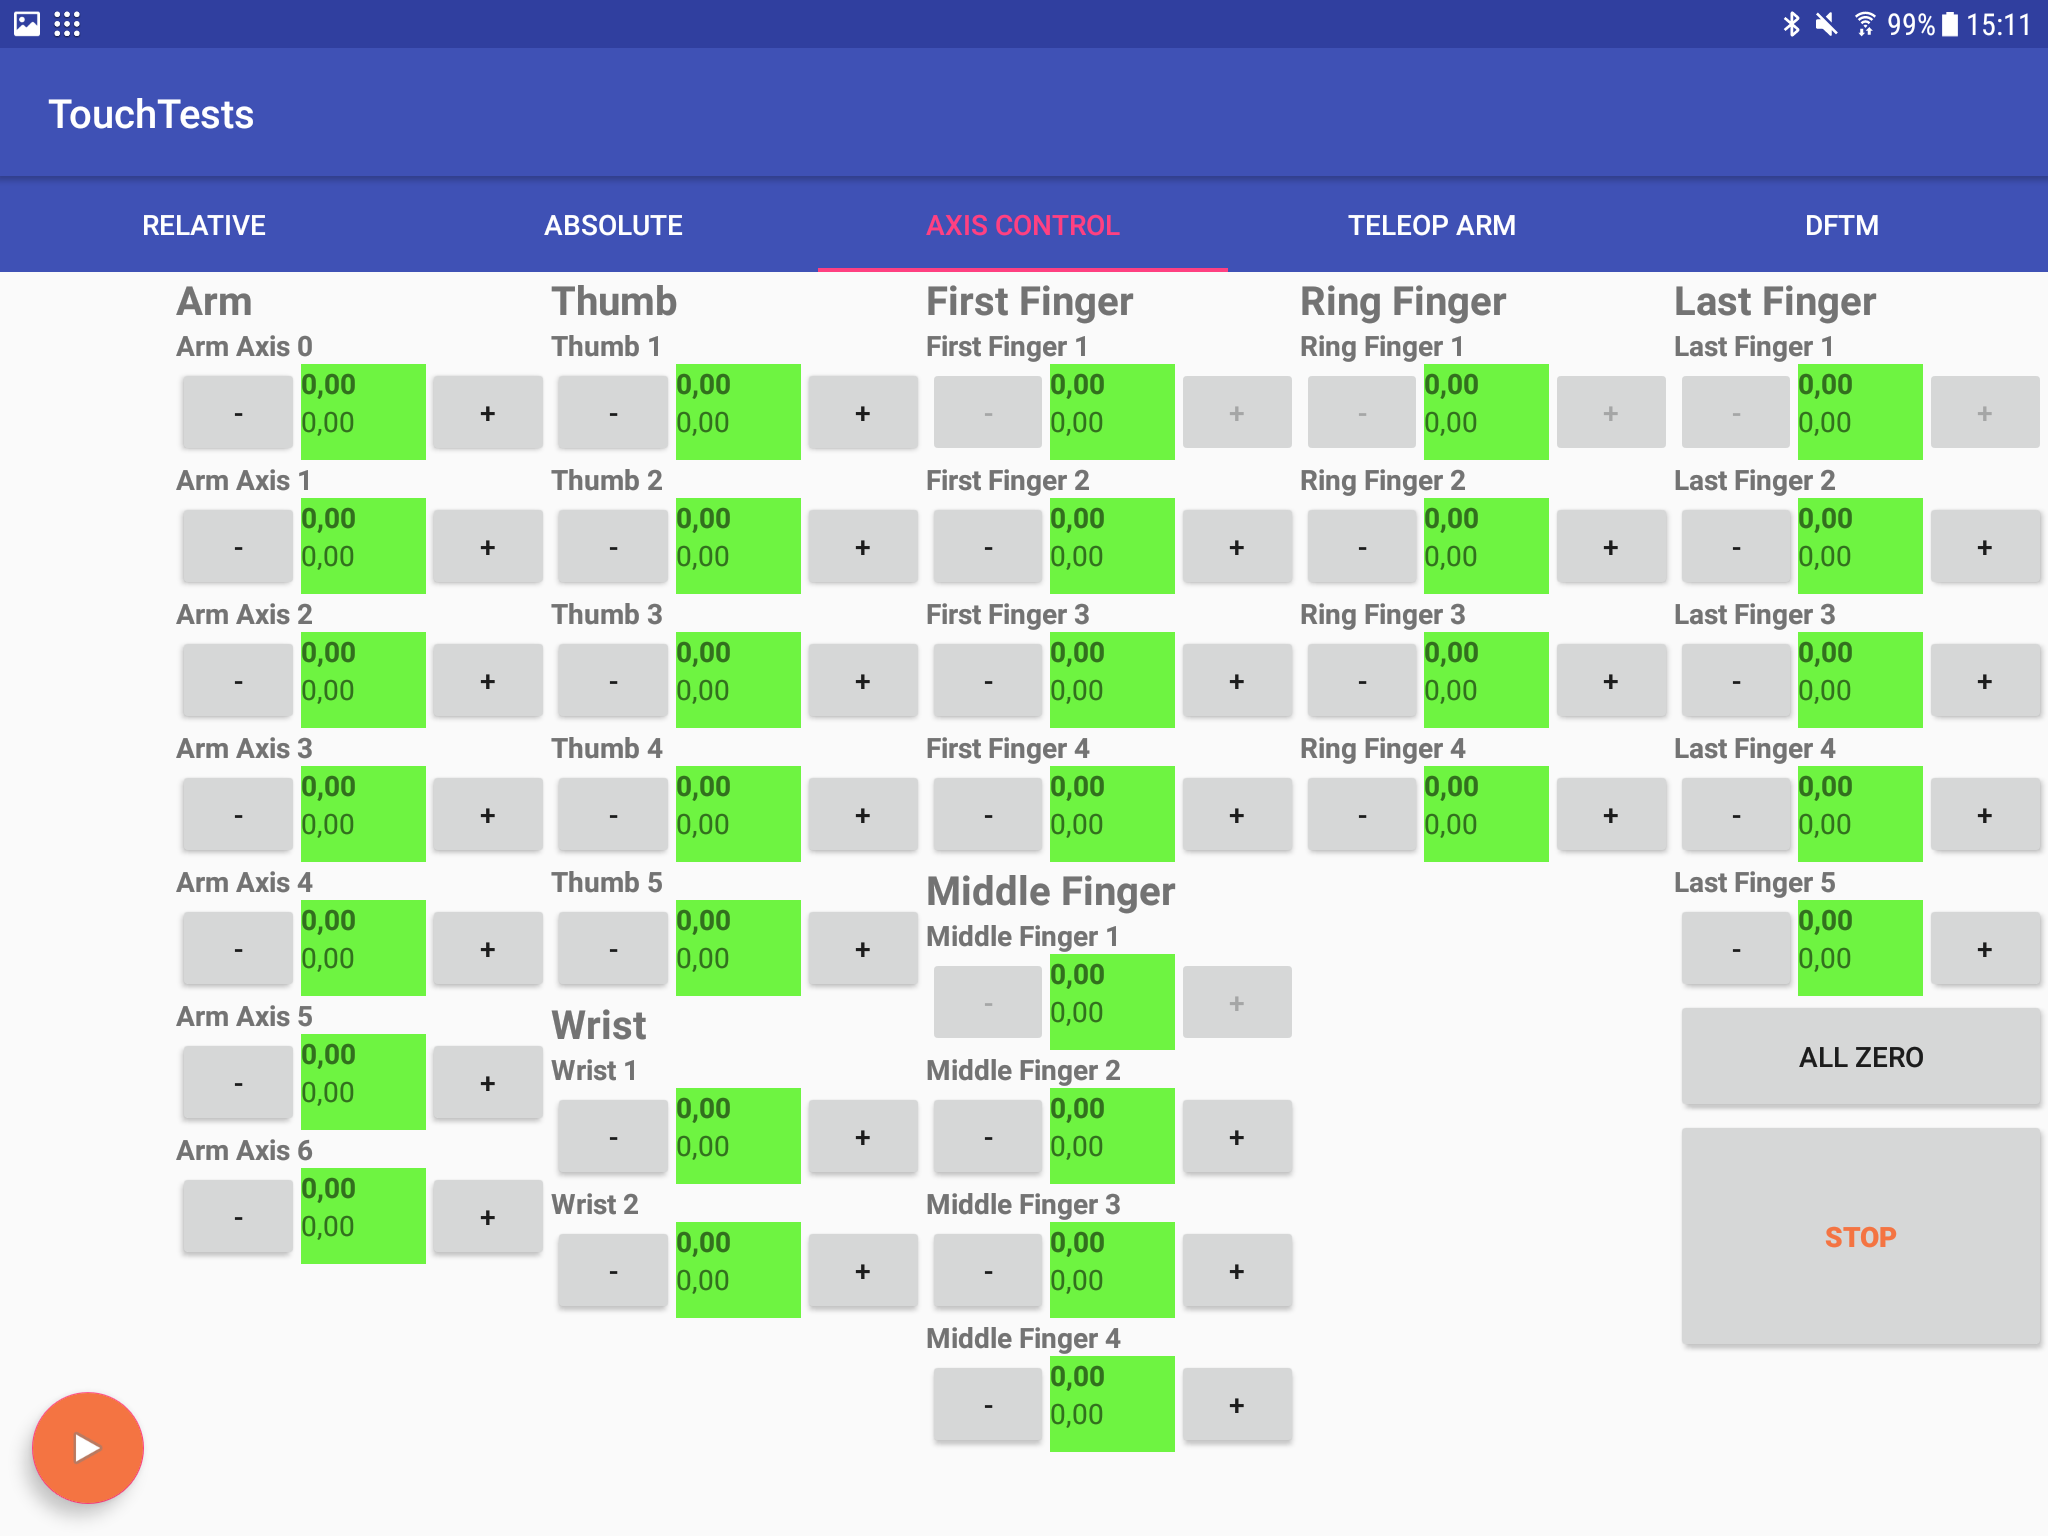
\includegraphics[width=0.75\linewidth]{assets/chpt_impl/axis_control.png}}
\end{figure}
\end{frame}

\begin{frame}{Arm Teleop}
\begin{figure}
	\boxed{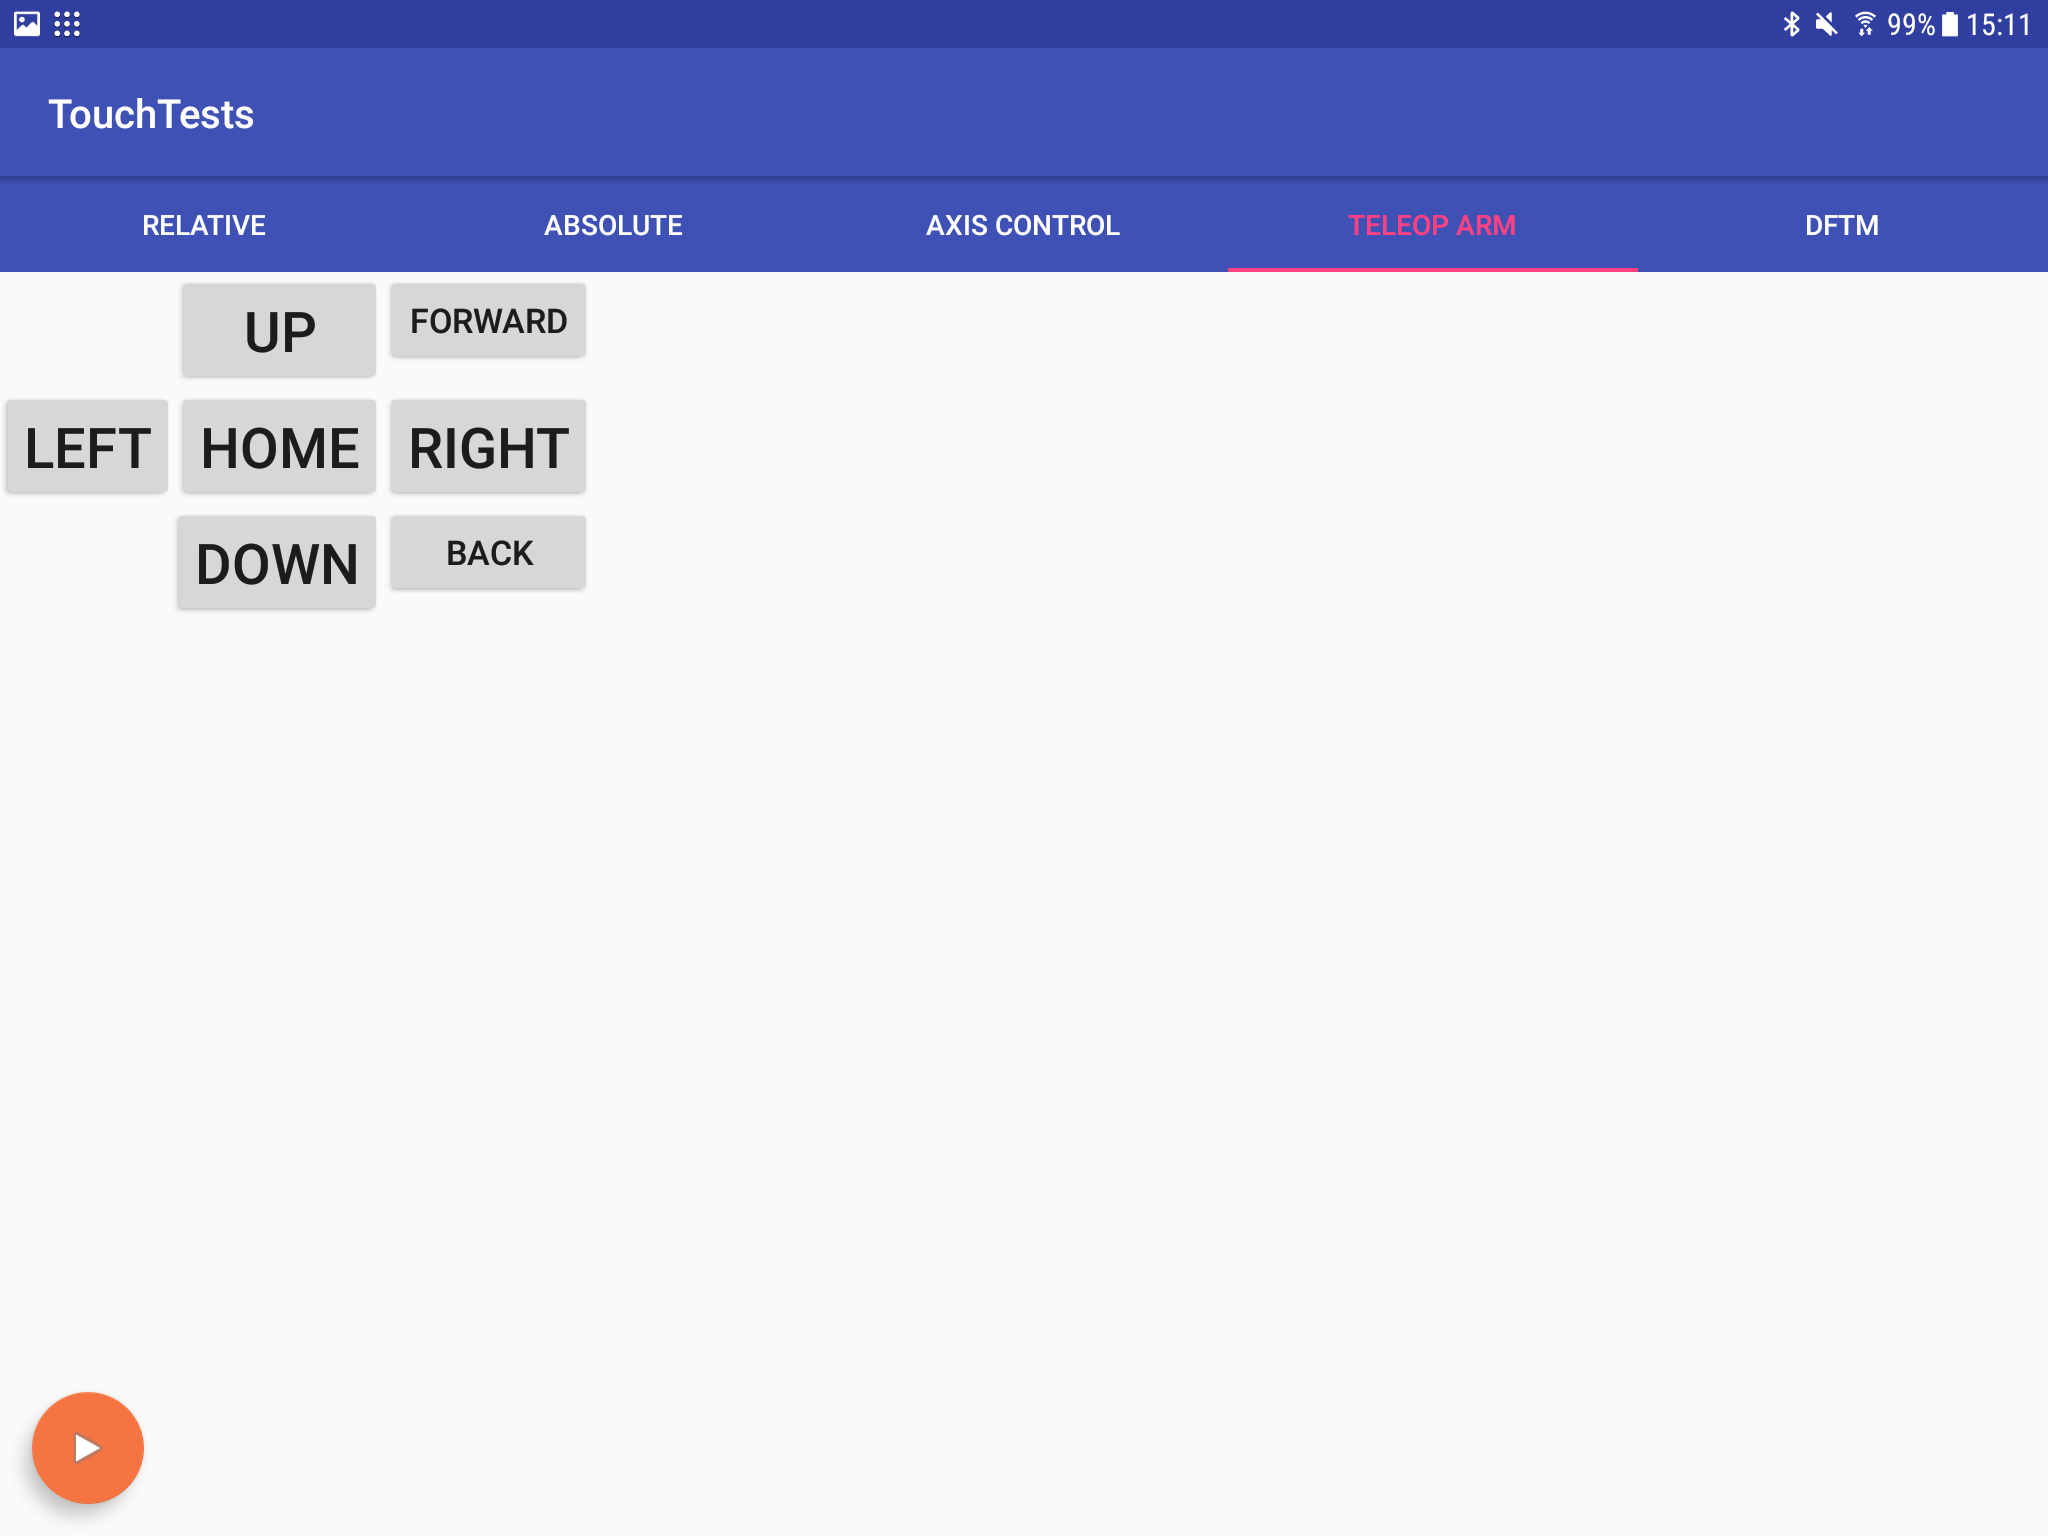
\includegraphics[width=0.75\linewidth]{assets/chpt_impl/teleop.png}}
\end{figure}
\end{frame}

\section{Implementation}
\subsection{Software Architecture}

\begin{frame}{Software Architecture}
\begin{itemize}
	\item \textit{Model-View-Controller} \cite{Eilebrecht2013}
	\item Model: \textit{AxisManager}, \textit{C5LwrNode}
	\item View: \textit{*View}
	\item Controller: \textit{*Proxy, *Fragment}, \textit{CartesianArmManager}
\end{itemize}
\end{frame}

\begin{frame}{Model-View-Controller}
\begin{figure}
	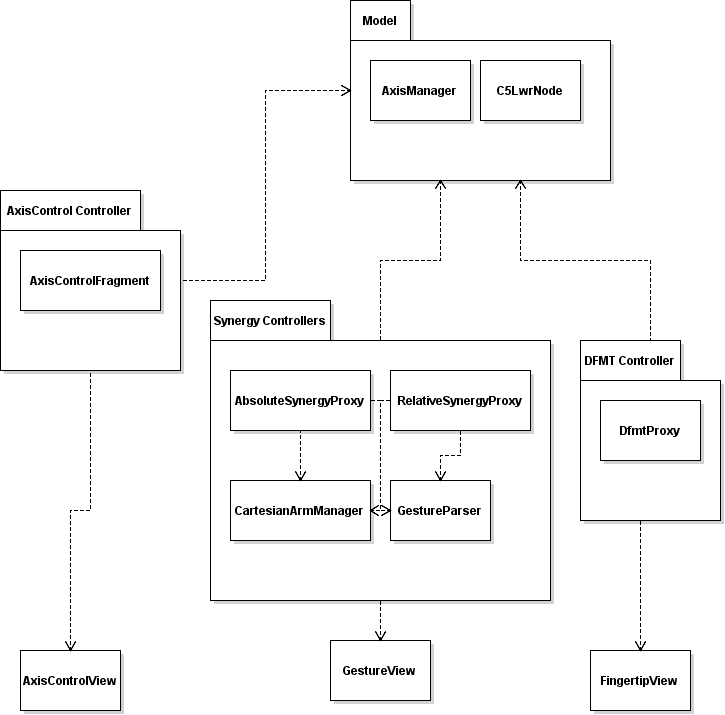
\includegraphics[width=0.6\linewidth]{assets/chpt_concepts/sw/mvc}
\end{figure}
\end{frame}

\begin{frame}{AxisManager}
\begin{itemize}
	\item \textit{Model} $\Rightarrow$ responsible for all joint data and movement
	\item Enable / Disable (Safety Interlock)
	\item Joint Movements
	\item Target Values
	\item Maximum Speed
\end{itemize}
\end{frame}

\begin{frame}{C5LwrNode}
\begin{itemize}
	\item Interface to ROS
	\item Receives joint information
	\item Sends joint information from AxisManager
	\item Methods to call the BioIK service
\end{itemize}
\end{frame}

\subsection{Synergy Approach}

\begin{frame}[fragile]{GraspSynergy}
\begin{itemize}
	\item $\theta = s_0 + S\alpha$
	\item $s_0$ and $S$ provided as data files
	\item Functionality to load data files and calculate joint angles in \textit{GraspSynergy} class (provided by Norman)
	\item Amplitudes range from $-50$ to $50$
\end{itemize}
\begin{lstlisting}
class GraspSynergy {
	public void parseMatlabSynergyMean(InputStream is);
	public void parseMatlabSynergyVecs(InputStream is);
	
	public double[] toJoints(double[] amplitudes);
}
\end{lstlisting}
\end{frame}

\begin{frame}{Touch Gestures}
\begin{itemize}
	\item Gesture property $\Rightarrow$ amplitude (relative or absolute)
	\item Position (Center)
	\item Size
	\item Orientation
\end{itemize}
Definitions:
\begin{itemize}
	\item $p = (p_x, p_y) \in \mathbb{R}^2$ is a \textbf{Pointer} on a touch screen
	\item $G = \{p_1,\dots , p_n\}$ for pointers $p_i,\,1 \leq i \leq n$ and $|G| \geq 1$ is a \textbf{Gesture}
\end{itemize}
\end{frame}

\begin{frame}{Gesture Properties}
For a gesture $G = \{p_1,\dots,p_n\}$
\begin{itemize}
	\item Position: \begin{equation}
	c(G) = \frac{1}{|G|}\sum_{i=1}^{|G|}p_i \qquad  p_i \in G
	\end{equation}
	
	\item Size: \begin{equation}
	s(G) = \frac{2}{|G|}\sum_{i=1}^{|G|} d(c(G), \, p_i)
	\end{equation}
	with $d(x, y) = \sqrt{(y_1 - x_1)^2 + (y_2 - x_2)^2}\,$ for $x, y \in \mathbb{R}^2$
\end{itemize}
\end{frame}

\begin{frame}{Gesture Properties}
For a gesture $G = \{p_1,\dots,p_n\}$

\begin{itemize}
	\item \textit{Thumb Pointer}:
	{\footnotesize
	\begin{equation}
	th(G) = \left\{
	\begin{array}{ll}
	p_1 & |G| = 1 \\
	p_n \text{ with } p_{n,y} = max\{p_{i,y} : p_i \in G\} & |G| = 2 \\
	p_n \text{ with } d(c(G), p_n) = max\{ d(c(G), p_i) : p_i \in G \}& |G| > 2
	\end{array}
	\right.
	\end{equation}}

	\item Orientation, for $v = c(G) - th(G)$,  $b_y = \vectwo{0}{-1}$:
	\begin{equation}
	\label{eq:conc:orientation}
	o(G) = \textnormal{sign}(\det(b_y\, v)) \cdot \arccos\left(\frac{v \cdot b_y}{|v| \cdot |b_y|}\right) \, .
	\end{equation}	

	\item $-\pi \leq o(G) \leq \pi $
\end{itemize}

\end{frame}

\begin{frame}{Gesture Example}
\begin{figure}
	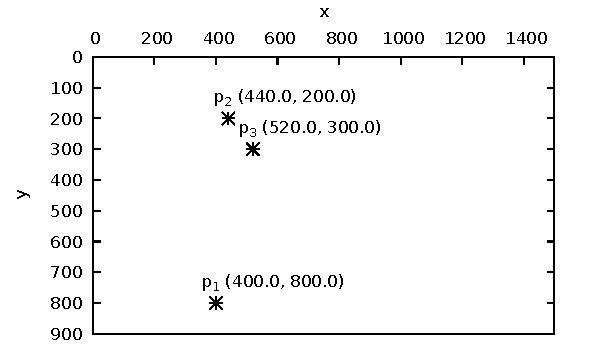
\includegraphics[height=0.8\textheight]{assets/chpt_concepts/gestures/3pointers_blank.pdf}
\end{figure}
\end{frame}

\begin{frame}{Gesture Example}
\begin{minipage}{0.5\linewidth}
	\begin{figure}
		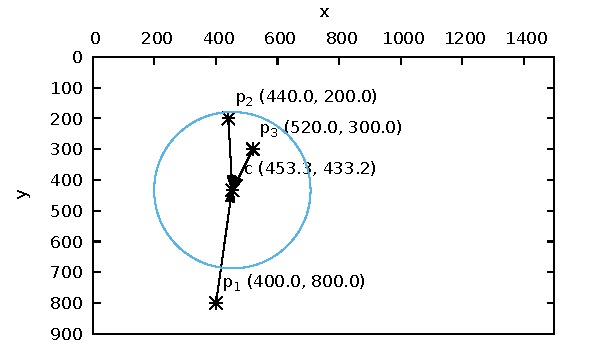
\includegraphics[width=\linewidth]{assets/chpt_concepts/gestures/3pointers_center.pdf}
	\end{figure}
\end{minipage}
\begin{minipage}{0.48\linewidth}
	\begin{itemize}
		\item $c(G) \approx \vectwo{453.3}{433.2}$
		\item $s(G) \approx 508.8$
		\item $o(G) \approx 0.141398 \, \widehat{\approx} \, 8.101 ^\circ$
	\end{itemize}
\end{minipage}
\end{frame}

\begin{frame}[fragile,allowframebreaks]{Implementation}
\footnotesize
\begin{itemize}
	\item \textit{Location} is a 2D vector
	\item \textit{Pointer} has a \textit{Location} and ID
	\item \textit{Gesture} has multiple \textit{Pointer}s
\end{itemize}

\begin{lstlisting}
public class Location {
	public Location(float x, float y);
	
	public float getX();
	public float getY();
	
	public Location add(Location loc);
	public Location substract(Location loc);
	public Location multiply(float c);
	public Location divide(float c);
	
	public double scalarProduct(Location loc);
	
	public double getVectorLength();
	public double distanceTo(Location loc);
	public double getAngleTo(Location loc);
	public Location getTurned(double angleRad);
}
\end{lstlisting}
\begin{lstlisting}
public class Gesture {
	public void addPointer(Pointer p);
	public void removePointer(Pointer p);
	public int getPointerCount();
	
	public Location getCenter();
	public float getSize();
	public double getOrientation();
}
\end{lstlisting}
\end{frame}

\begin{frame}{Gesture Visualization}
\begin{figure}
	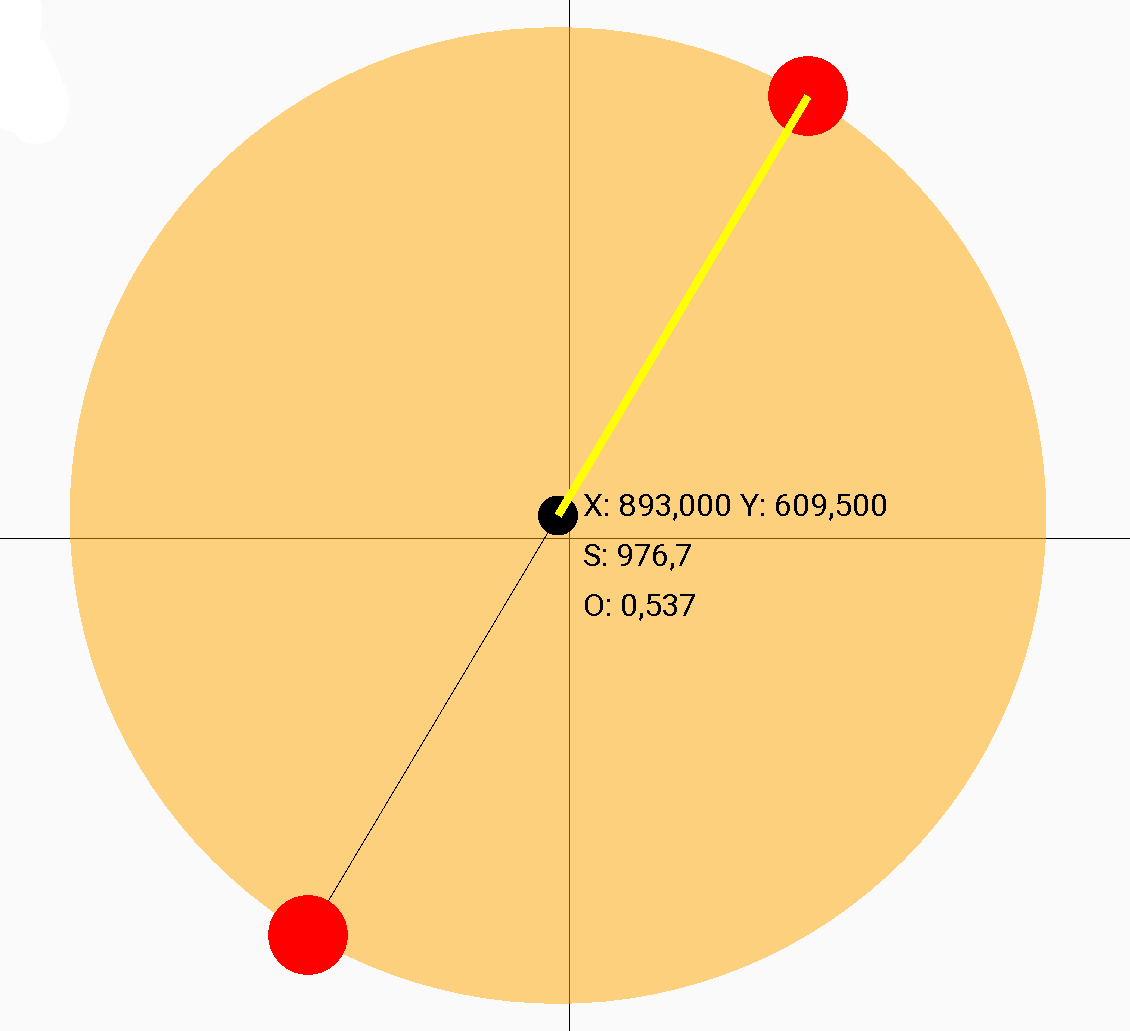
\includegraphics[height=0.7\textheight]{assets/chpt_impl/syn_2touch}
	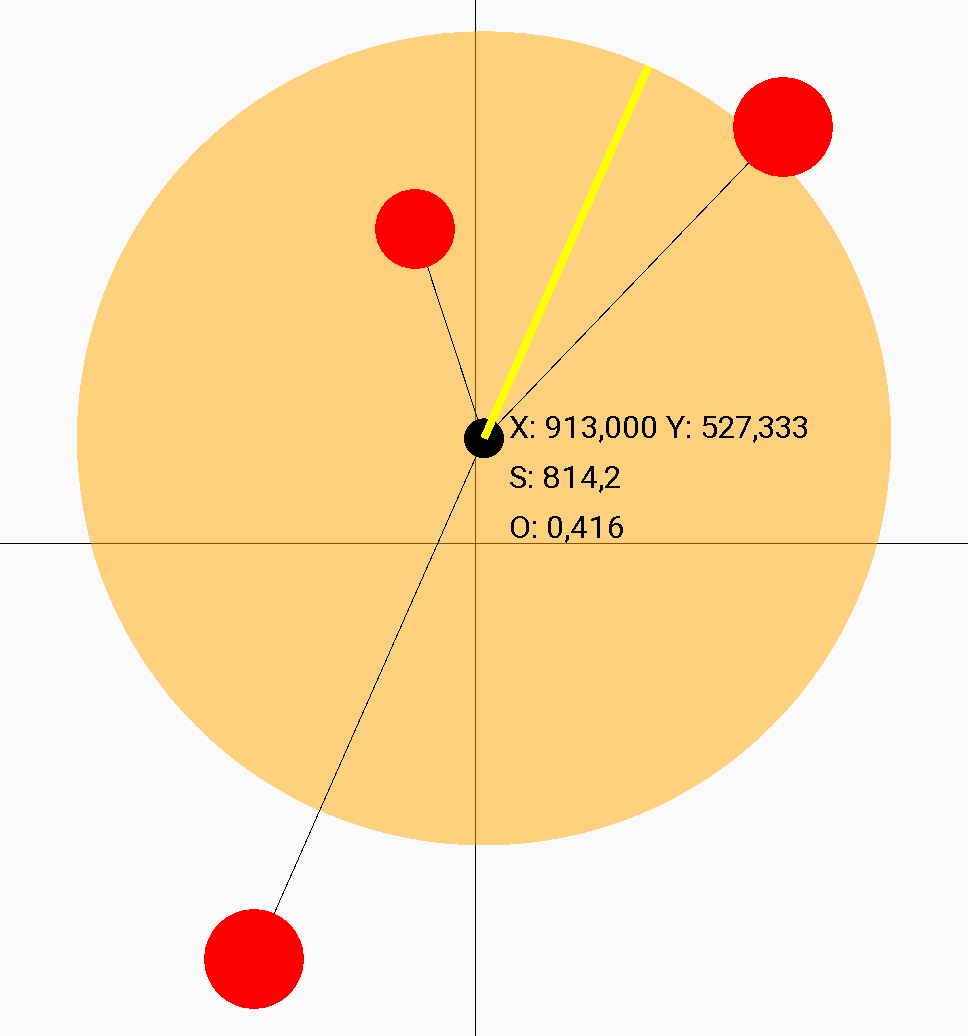
\includegraphics[height=0.7\textheight]{assets/chpt_impl/syn_3touch}
\end{figure}
\end{frame}

\begin{frame}{AbsoluteSynergyProxy}
\begin{itemize}
	\item Maps gesture properties linearly ti amplitude values
	\item Maps gesture properties to robot palm position
	\item Gesture with two pointer used for amplitude control
\end{itemize}

\begin{figure}
	\begin{tabular}{|c|r|c|c|}
	\hline
	\textbf{\#} & \textbf{Property} & \textbf{50 at} & \textbf{-50 at} \\
	\hline
	1 & $s(G)$ & 1200 & 300 \\
	\hline
	2 & $c(G)_1$ & $0.25\cdot\text{screenwidth}$ & $0.75\cdot\text{screenwidth}$\\
	\hline
	3 & $o(G)$ & $-\frac{\pi}{2}$ & $\frac{\pi}{2}$ \\
	\hline	
	\end{tabular}
\end{figure}
\end{frame}

\begin{frame}{Arm Control}
\begin{itemize}
	\item \textit{CartesianArmManager}
	\item Accepts target positions for the C5 hand palm
	\item Requests IK solution for position endlessly
	\item When solution received: Set at \textit{AxisManager}
	\item 3-Pointer-Gestures are used for arm positioning
\end{itemize}

\begin{figure}
	\begin{tabular}{|c|c|c||c|c|c|}
		\hline
		\textbf{Axis} & \textbf{min} & \textbf{max} & \textbf{Prop.} & \textbf{min at} & \textbf{max at} \\
		\hline
		X & -0.2 & 0.4 & $c(G)_1$ & $0.25 \cdot \text{screenwidth}$ & $0.75\cdot \text{screenwidth}$  \\
		\hline
		Z & 1.10 & 1.35 & $c(G)_2$ & $0.75 \cdot \text{screenheight}$ & $0.25\cdot \text{screenheight}$ \\
		\hline
	\end{tabular}
\end{figure}

\end{frame}

\begin{frame}{Arm Coordinate System}
\begin{figure}
	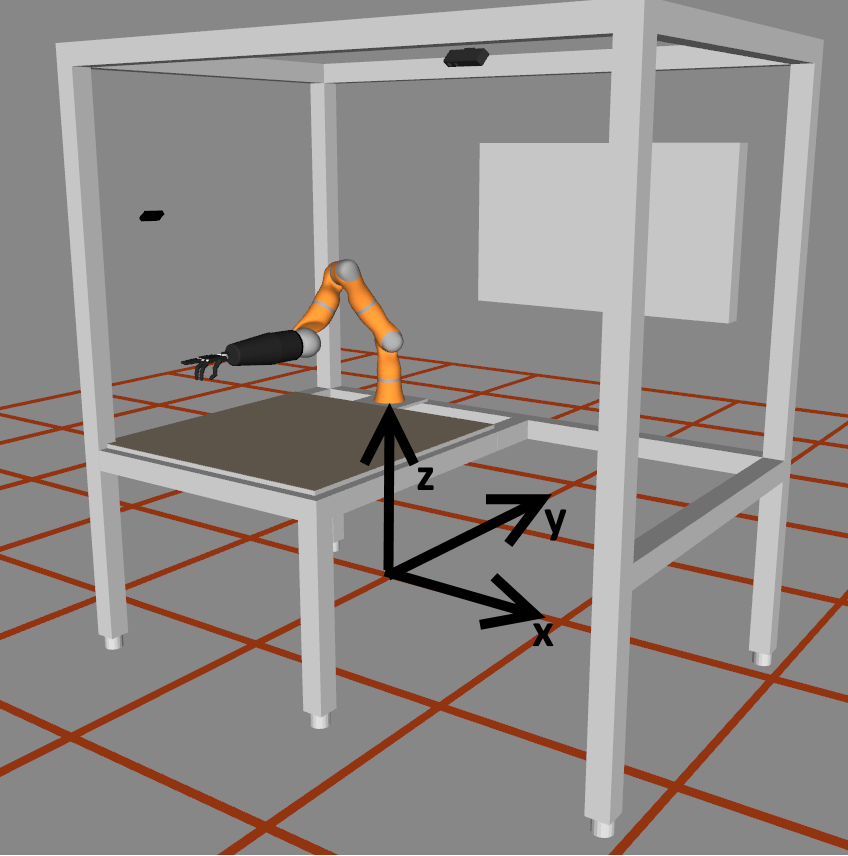
\includegraphics[height=0.8\textheight]{assets/chpt_concepts/coordinates}
\end{figure}
\end{frame}

\begin{frame}{RelativeSynergyProxy}
\begin{itemize}
	\item Very similar to absolute mapping
	\item Mapping from property to Amplitude/Axis same
	\item Rate of change stored for every mapping
	\item Current value is altered
\end{itemize}
\end{frame}

\subsection{Direct Fingertip Mapping}

\begin{frame}{Direct Fingertip Mapping}
\begin{itemize}
	\item \textit{DFTM}
	\item Mapping fingertips from touch screen to a plane in 3D space
	\item Relative positions of fingertips equal
	\item Plane in 3D space:
	\begin{equation}
	E:\vec{p} = \vec{b} + x \cdot \vec{e_1} + y \cdot \vec{e_2}
	\end{equation}
	\item $|\vec{e_1}| = |\vec{e_2}| = 1$ (1m)
\end{itemize}
\end{frame}

\begin{frame}{Direct Fingertip Mapping}
\begin{figure}
	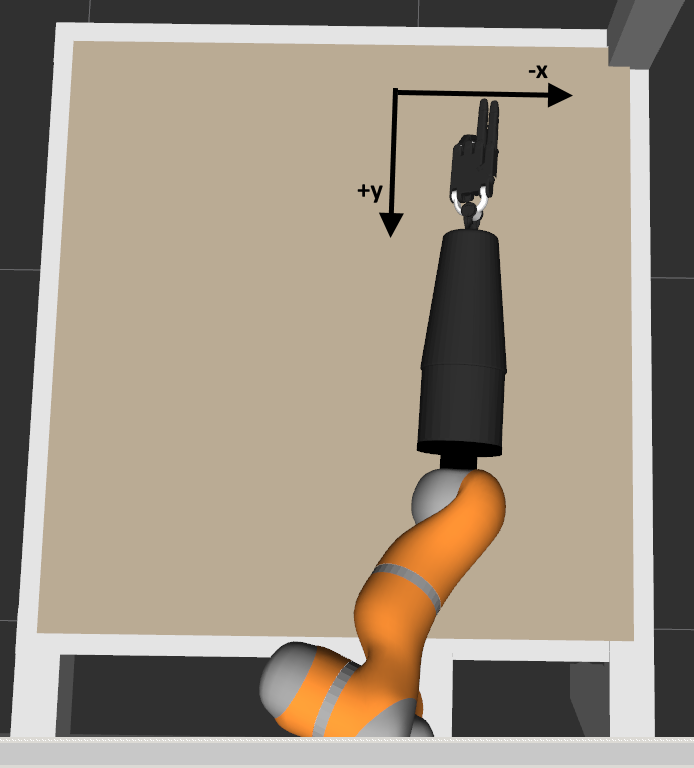
\includegraphics[height=0.55\textheight]{assets/chpt_concepts/dfmt_coord_arm}
	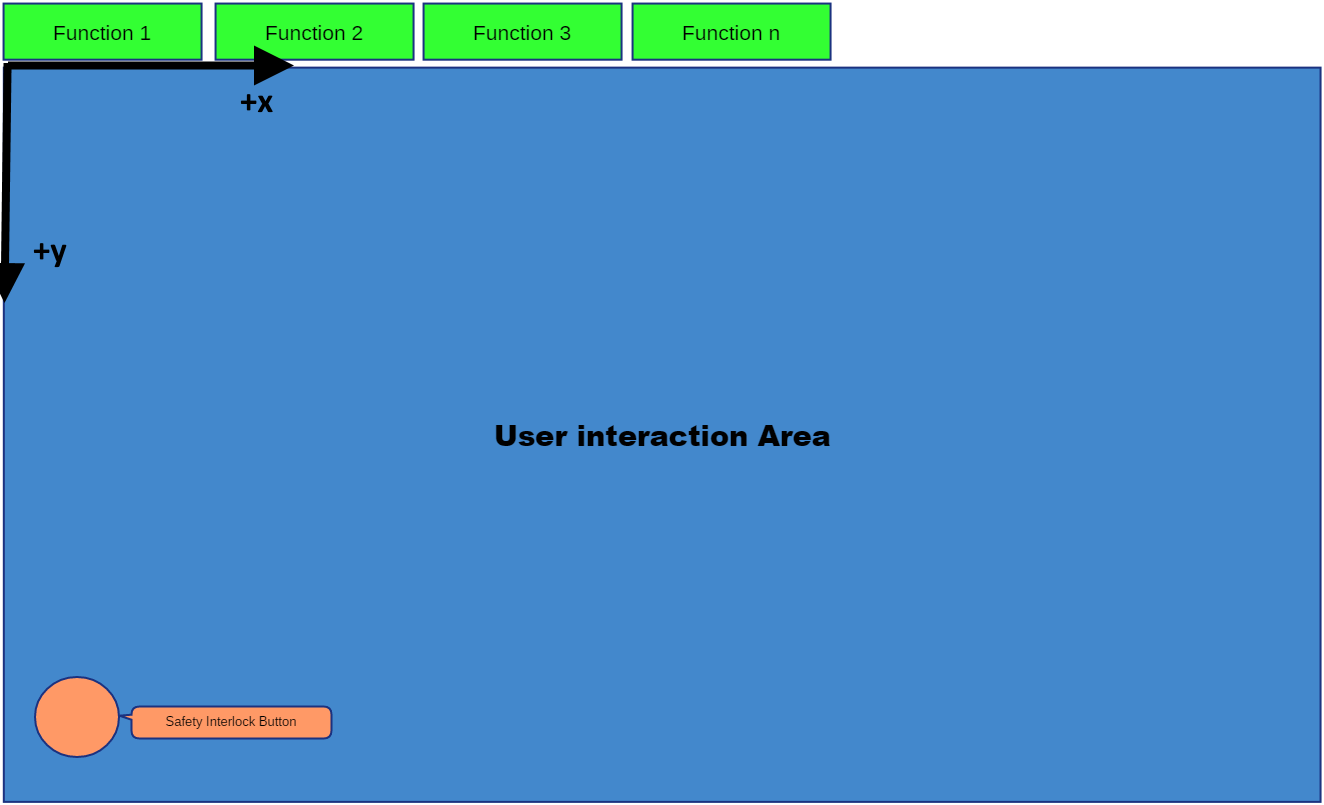
\includegraphics[height=0.55\textheight]{assets/chpt_concepts/dfmt_coord_screen}
\end{figure}
\end{frame}

\begin{frame}{DFTM Parameters}
\begin{itemize}
	\item $\vec{b} = \vecthr{0}{-1.25}{1.2}$
	\item $\vec{e_1} = \vecthr{-1}{0}{0}$
	\item $\vec{e_2} = \vecthr{0}{1}{0}$
\end{itemize}
\end{frame}

\begin{frame}{DFTM Screen}
\begin{figure}
	\boxed{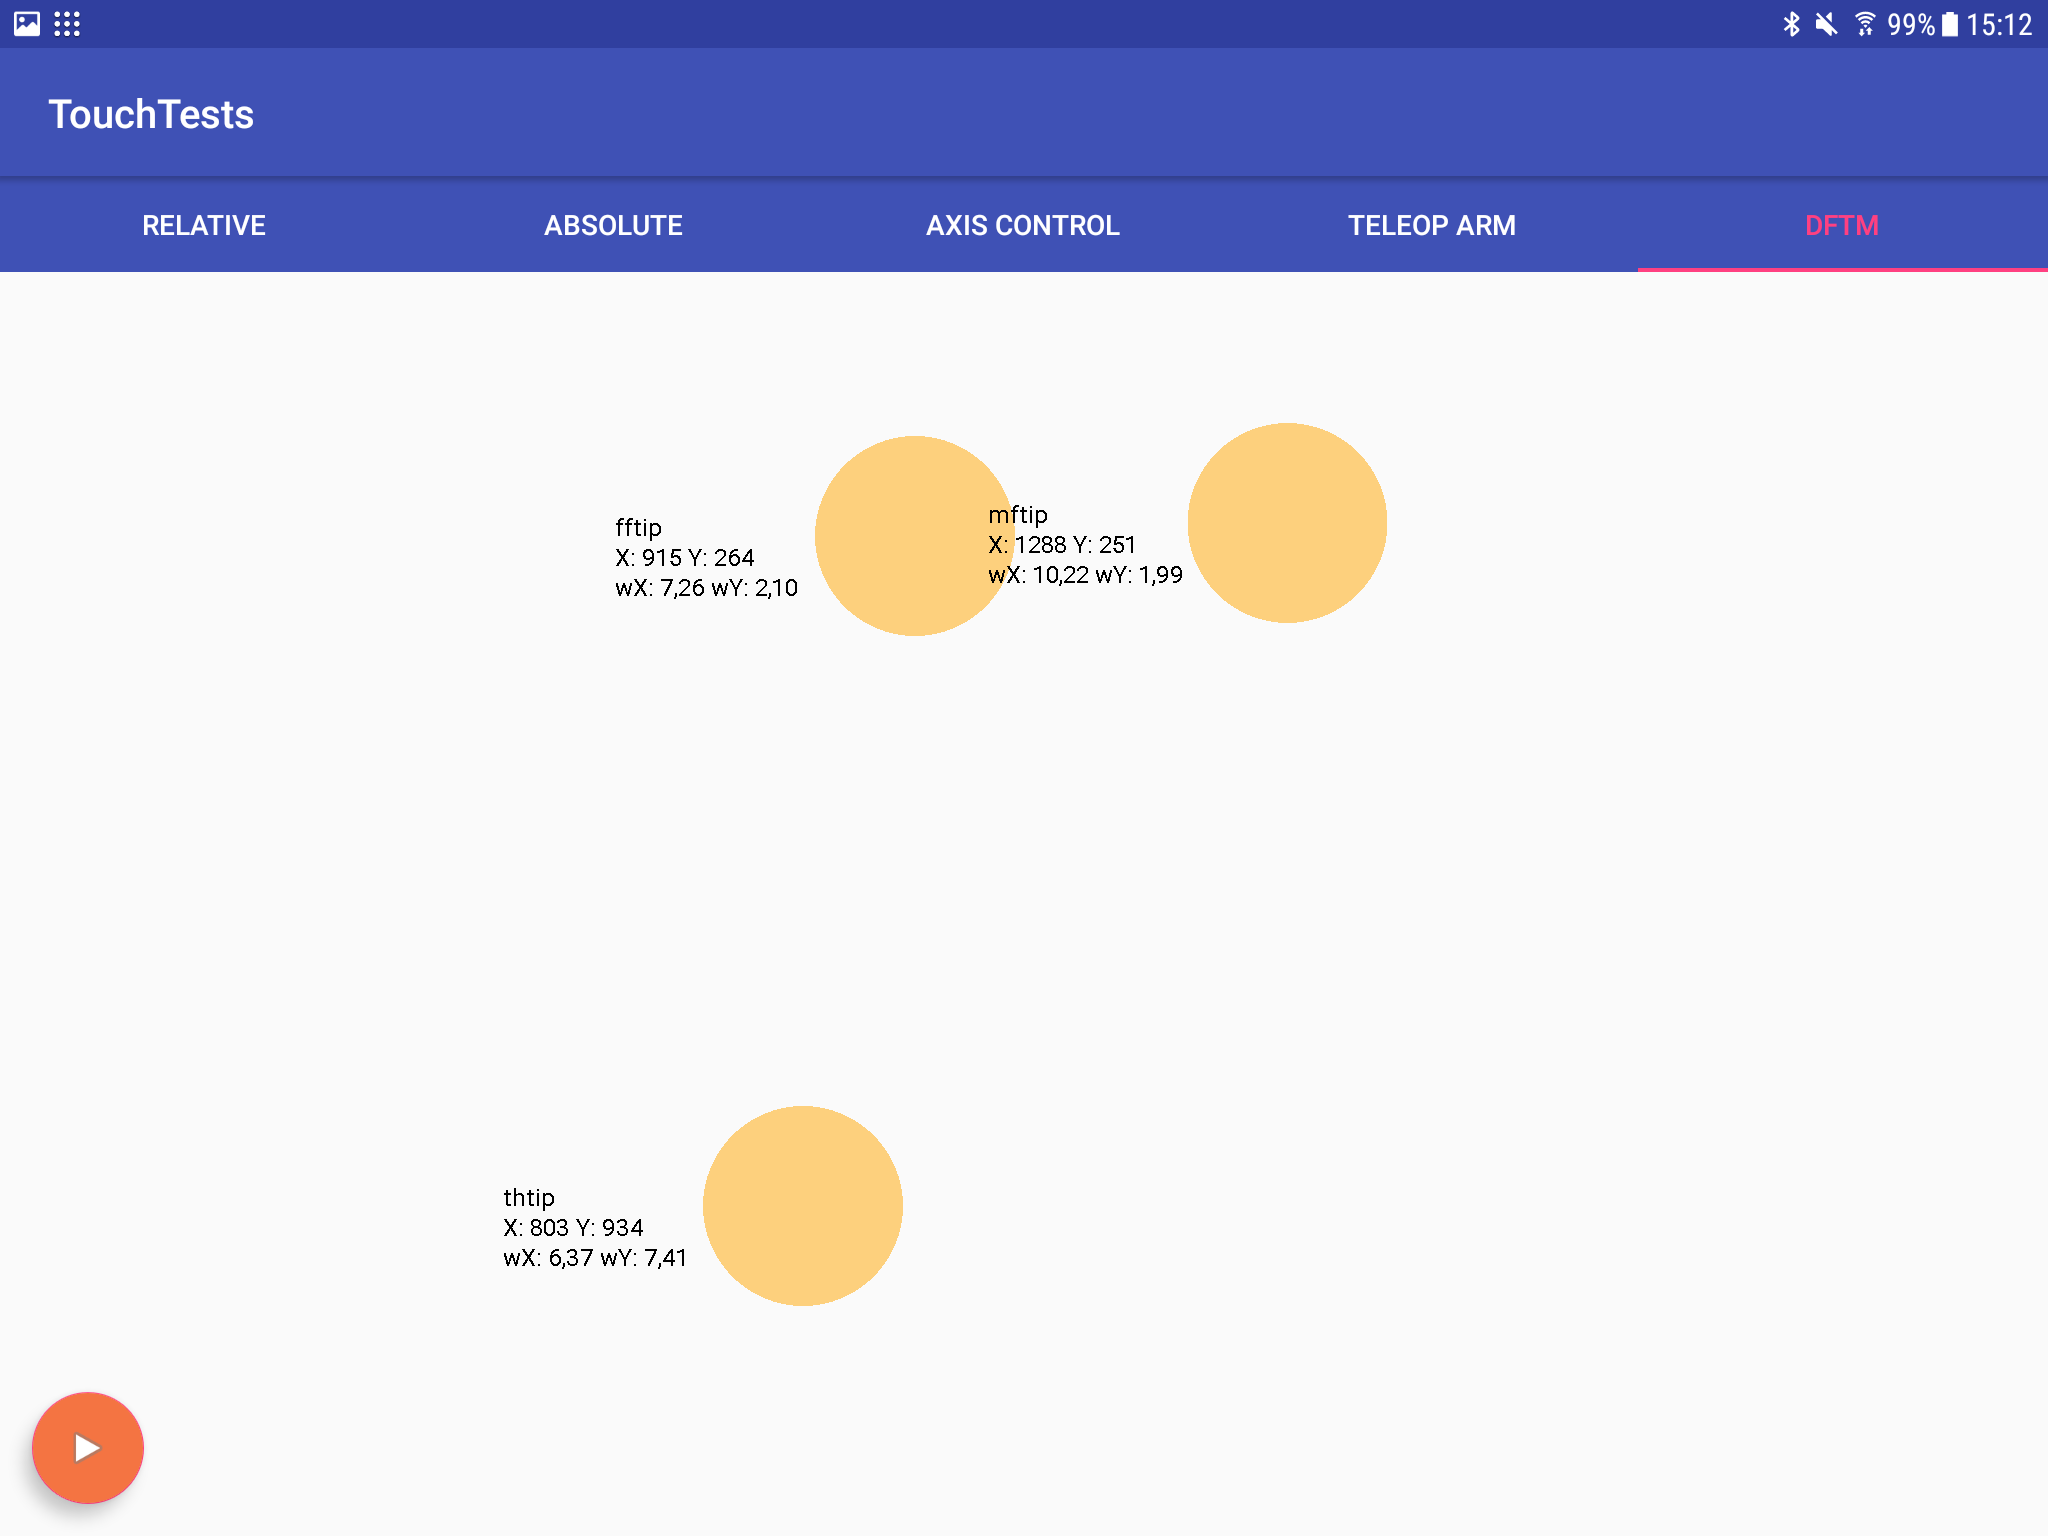
\includegraphics[height=0.78\textheight]{assets/chpt_impl/dftm}}
\end{figure}
\end{frame}

\begin{frame}{DFTM Screen}
\begin{figure}
	\boxed{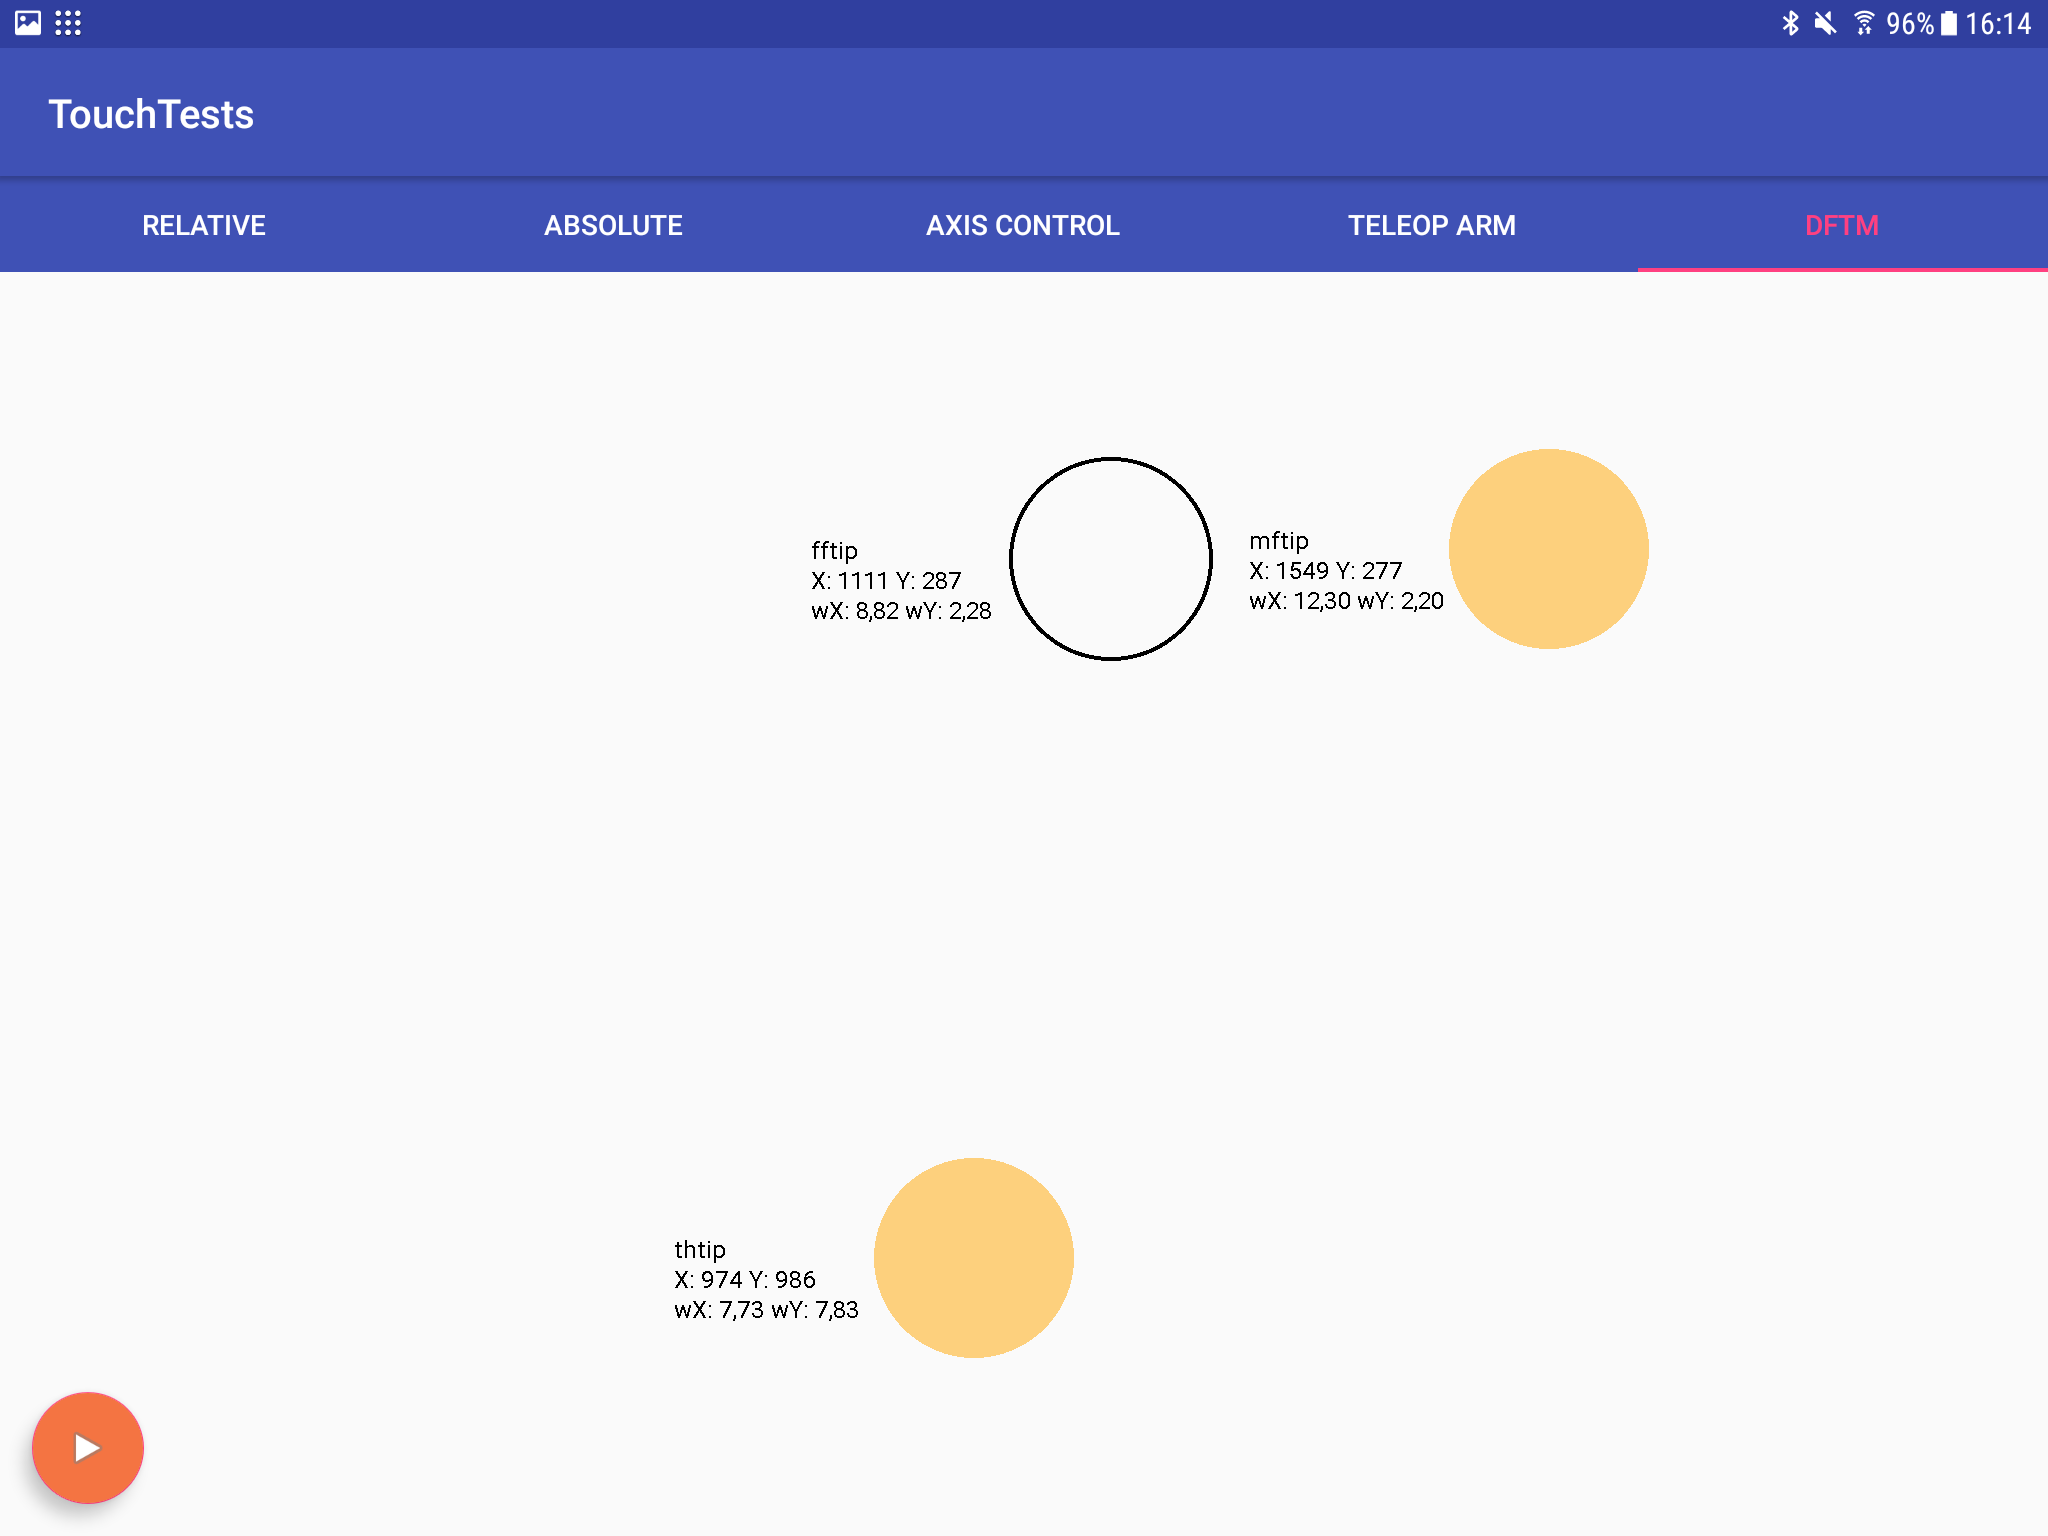
\includegraphics[height=0.78\textheight]{assets/chpt_impl/dftm_lifted}}
\end{figure}
\end{frame}

\subsection{Summary}

\begin{frame}{Summary}
\begin{itemize}
	\item Kuka LWR Arm + Shadow C5 Hand
	\item Relative Synergy Control
	\item Absolute Synergy Control
	\item Direct Fingertip Mapping Control
	\item on a 10" Android Tablet
\end{itemize}
\end{frame}

\section{Evaluation \& Outlook}

\begin{frame}{Evaluation}
\begin{itemize}
	\item Works as expected, in principle
	\item Synergy control is fine
	\item Unwanted arm movements when gesture is stationary
	\item BioIK seems to return a different / new solution for the same position
	\item Jittering even more disturbing in DFTM mode
	\item $\Rightarrow$ \textit{MinimumDisplacementGoal} helps, slows down IK
\end{itemize}
\end{frame}

\begin{frame}{Performance}
\begin{itemize}
	\item Application overall performance is good
	\item Device gets warm $\Rightarrow$ constant network flow with small packages
	\item Service calls in \textit{rosjava} / \textit{rosandroid} designed to be asynchronous, but UI blocked during service calls
	\item Service calls to the BioIK service take long
\end{itemize}
\end{frame}

\begin{frame}{BioIK Service Performance (1000ms timeout)}
\begin{figure}
	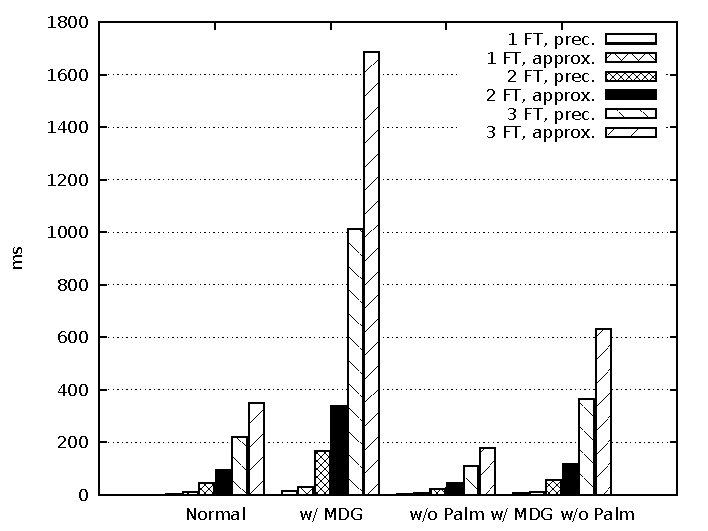
\includegraphics[height=0.8\textheight]{assets/chpt_eval/1000ms.pdf}
\end{figure}
\end{frame}

\begin{frame}{BioIK Service Performance (10ms timeout)}
\begin{figure}
	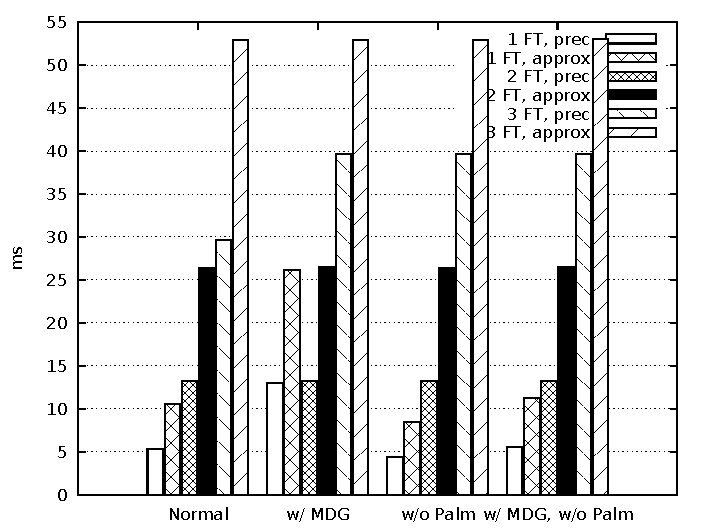
\includegraphics[height=0.8\textheight]{assets/chpt_eval/10ms.pdf}
\end{figure}
\end{frame}

\begin{frame}{Conclusions}
\begin{itemize}
	\item BioIK uses the time it is given \cite{Ruppel17}
	\item IK frequency doesn't rise significantly in application
	\item The BioIK service doesn't seem to be the problem
	\item Implementation of \textit{rosjava} / \textit{rosandroid} buggy?
\end{itemize}
\end{frame}

\begin{frame}{Future Work}
\begin{itemize}
	\item Look into performance issues
	\item Look into arm position jitter
	\item Implement user feedback (sound, visual, vibration)
	\item User Studies
\end{itemize}

\begin{itemize}
	\item Implement more approaches
\end{itemize}
\end{frame}

\section*{I'm done.}

\begin{frame}[c]
\centering
Thank you.
\end{frame}


\section{Bibliography}

\begin{frame}[allowframebreaks]{Bibliography}
\printbibliography
\end{frame}

\end{document}
